\section{Particles in the heliosphere}
\label{sec:particles_heliosphere}

Our heliosphere is an enormous region in space embedded in the \ac{ISM}, which encompasses all solar system planets and extends far beyond even the Kuiper belt. 
It is filled with a thin plasma consisting of various populations of particles, many of which originate from the Sun itself (\autoref{fig:heliospheric_energy_spectrum}). 
The most abundant population is the solar wind, a steady flow of plasma that is emitted from the Sun radially. 
In the near-Earth space, the slow solar wind reaches typical speeds between \SIrange[range-phrase={\,and\,}]{300}{500}{\kilo\meter\per\second}.
Due to its low pressure, and therefore high plasma $\beta$, it carries the solar magnetic field with it and forms the \ac{IMF}.
As the Sun rotates, the \ac{IMF} carried by the solar wind is shaped like an Archimedian spiral, which is named Parker spiral after Eugene N. \citet{Parker-1958}.

\begin{figure}
    \centering
    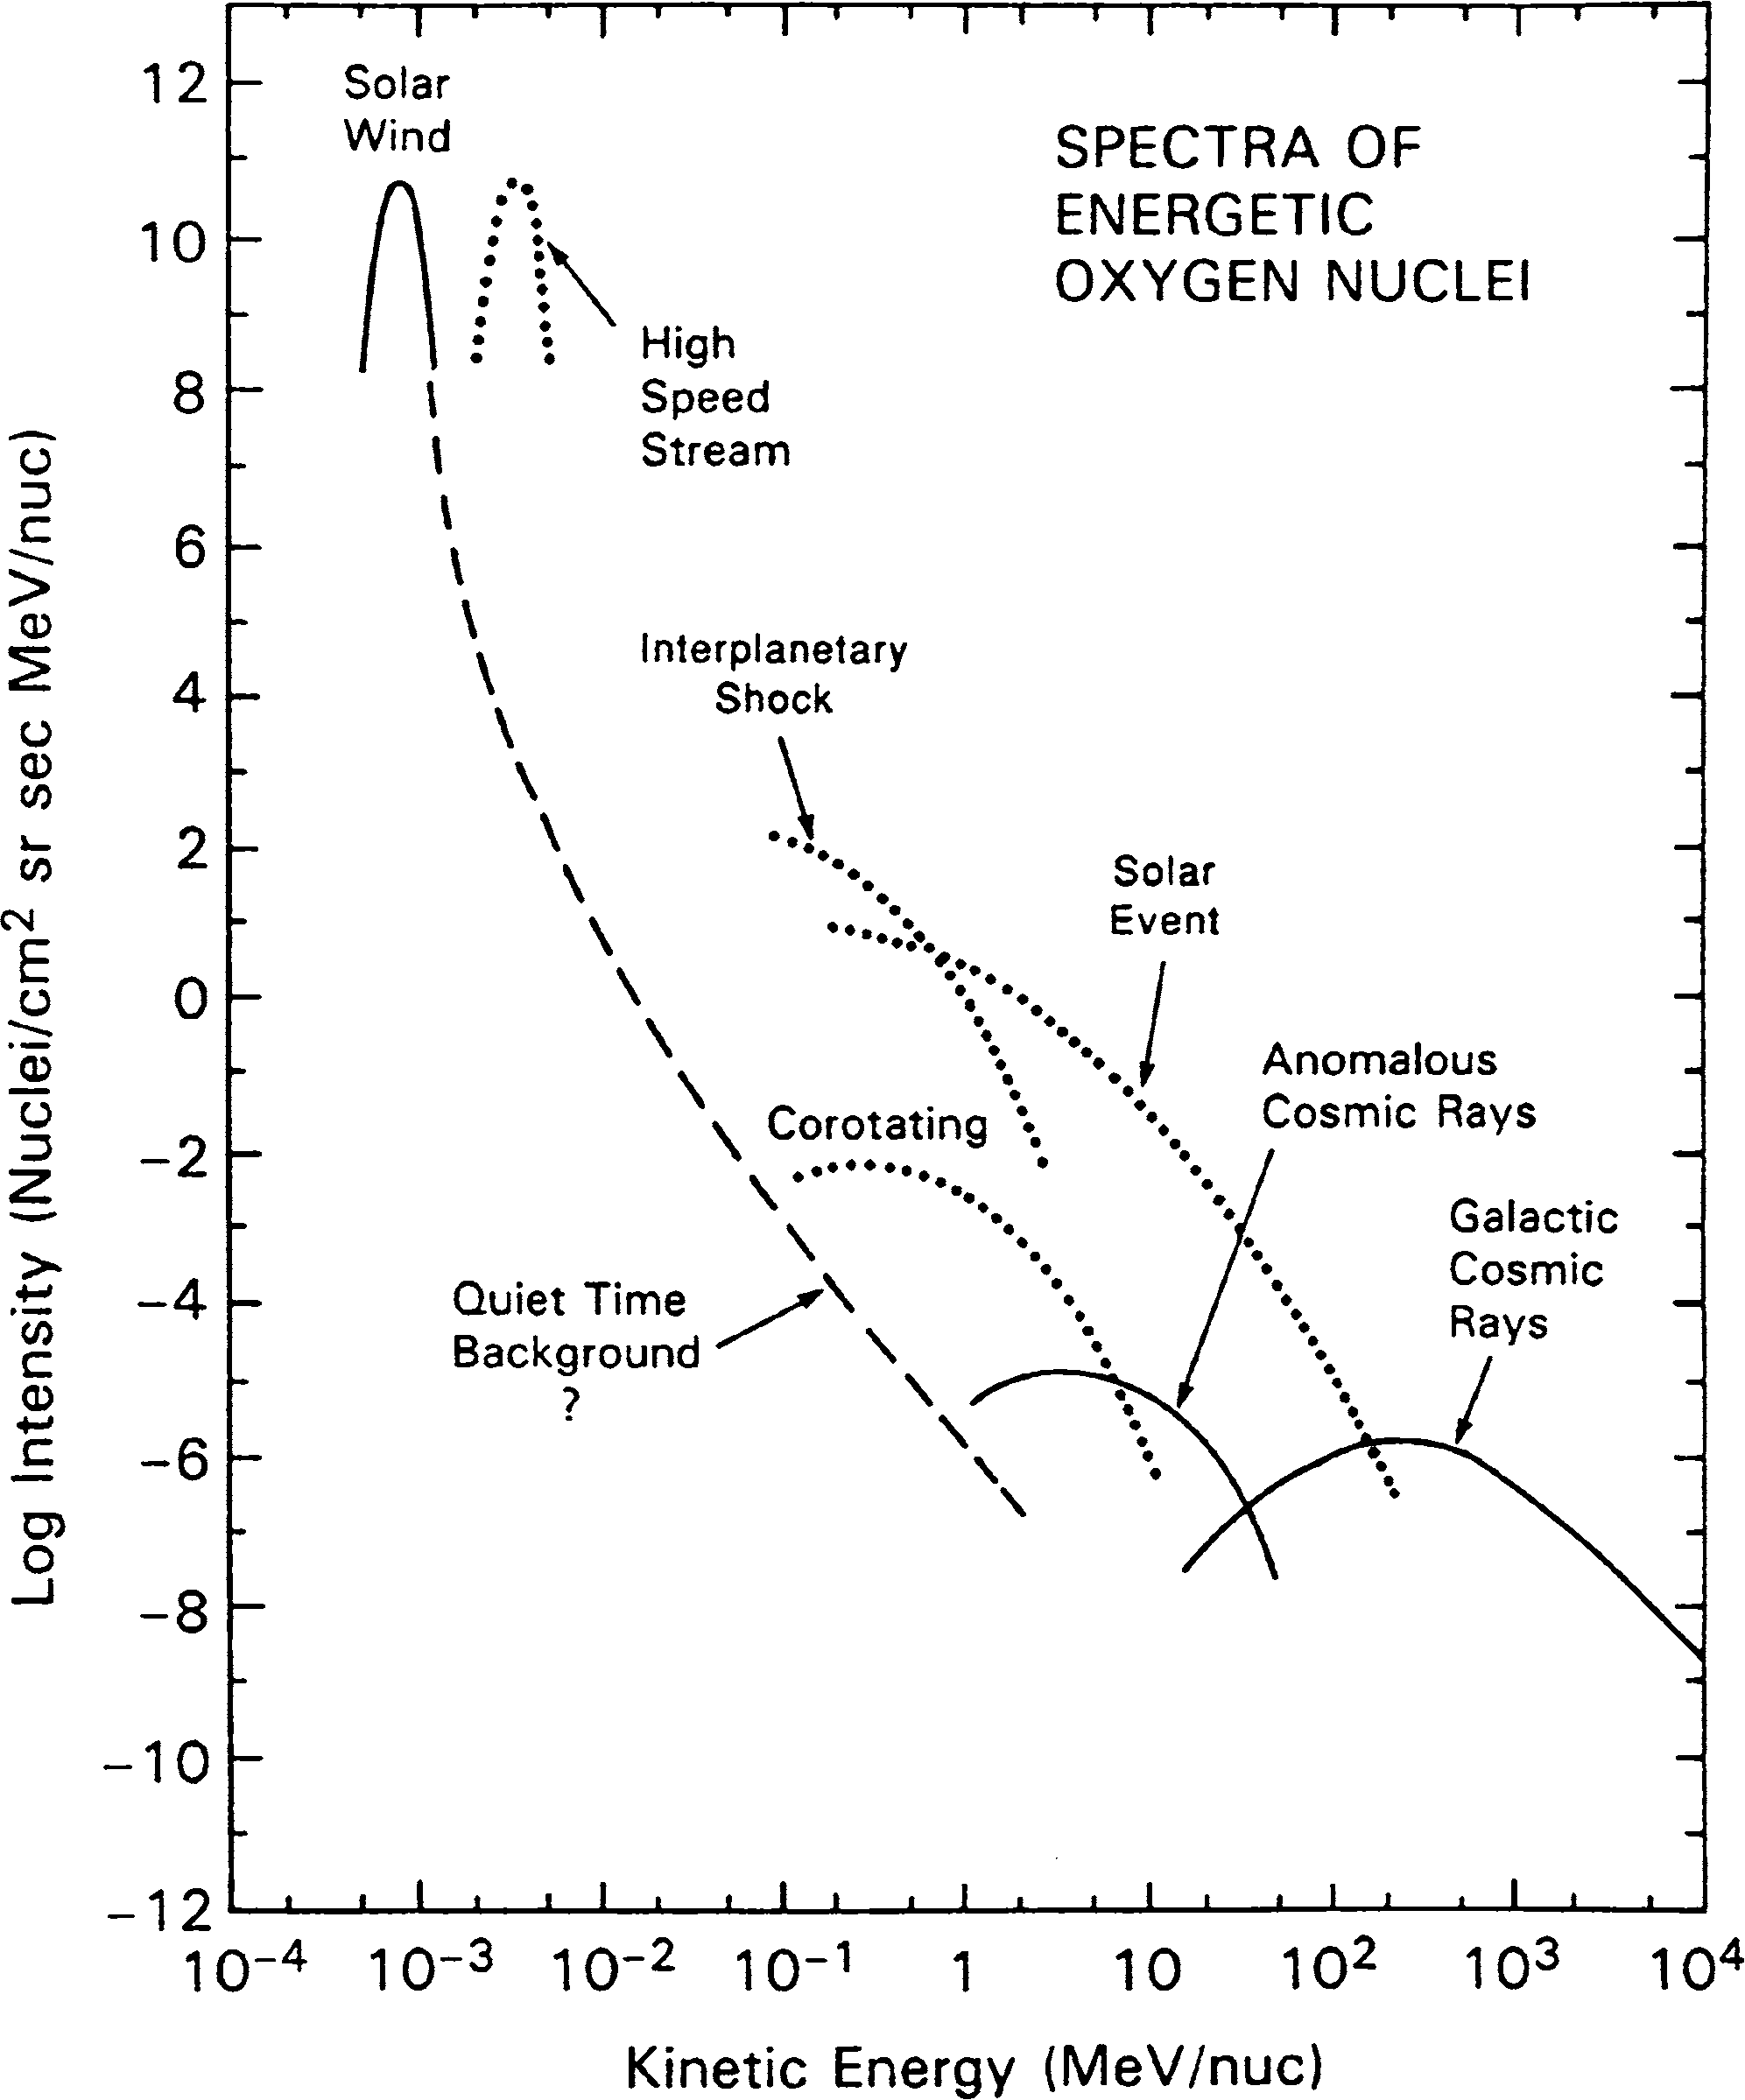
\includegraphics[width=0.6\linewidth]{images/heliospheric_energy_spectrum}
    \caption[Spectra of oxygen ions in the near-Earth interplanetary space]{Typical spectra of oxygen ions in the near-Earth interplanetary space, showing the contributions from different populations. Other particle species show similarly shaped spectra when plotted as a function of energy/nucleon. (adapted from \url{http://helios.gsfc.nasa.gov/ace/gallery.html}, based on \citet{Mewaldt-2001}).}
    \label{fig:heliospheric_energy_spectrum}
\end{figure}

However, our Sun is an active star, and thus, the flow of particles is not simply constant.
Coronal holes forming on the solar surface emit faster solar wind streams with speeds $\gtrsim \SI{600}{\kilo\meter\per\second}$, which interact with the neighboring streams of slower wind by forming a \ac{SIR}. If a coronal hole stays stable for multiple solar rotations, these interaction regions can be observed recurrently, in which case they are called \acp{CIR}.
Furthermore, active regions on the Sun can occasionally produce solar flares, sudden and intense emissions of light often associated with the release of high-energy ($\sim \si{\mega\electronvolt}$) \acp{SEP}.
These are believed to be powered by reconnection of magnetic field lines at the Sun, which leads to the release of energy and acceleration of particles.
They often also coincide with the eruption of plasma from the solar corona in the form of a \ac{CME} at speeds ranging from a few hundreds up to a few thousands of \si{\kilo\meter\per\second}.
Just like the solar wind, \acp{CME} carry a magnetic field with them, often in the form of a flux rope propagating away from the Sun. Due to their high speed, a shock can form in front of the flux rope, followed by a turbulent sheath region.
This shock can also be efficient at accelerating additional particles to higher energies, similar to \acp{SEP} particles accelerated directly at the Sun.

At the high end of the energy spectrum (\autoref{fig:heliospheric_energy_spectrum}) up to \si{\giga\electronvolt} energies, we find \acp{GCR}, particles originating from outside the heliosphere and entering it with a relatively constant and isotropic flux. 
The flux of these high-energy particles within the heliosphere is modulated by various effects: In the long term, the variation of the \ac{IMF} intensity during the 22-year solar cycle modulates the\ac{GCR} intensity observed in the inner solar system, so that the average \ac{GCR} flux is higher during solar minimum than at solar maximum \citep{Fisk-1980}. In addition, there are short-term modulations of \ac{GCR} due to magnetic structures in the solar wind, such as \acp{CME} and \acp{SIR}/\acp{CIR}. These are the so-called Forbush decreases, which will be the main focus of this thesis.

\section{Space Weather events and their detection}
\label{sec:spaceweather}

As defined by the U.S. National Space Weather Program \parencite{OFCM-1995}, the term \textit{space weather} refers to ``conditions on the Sun and in the solar wind, magnetosphere, ionosphere and thermosphere that can influence the performance and reliability of space-borne and ground-based technological systems and endanger human life or health''.
The aforementioned short-term heliospheric events, such as \acp{SEP}, \acp{CME} and \acp{CIR} are all relevant to space weather science, as both the increased radiation exposure due to accelerated energetic particles as well as the magnetic field disturbances, which impact spacecraft or impact the Earth's magnetosphere in a so-called magnetic storm, can have such impacts on technology or human life on Earth, in space, and on other planets.

Thus, the focus in space weather research is to enhance the understanding of these events in order to be able to more accurately predict their occurrence and propagation, including the onset time at Earth or other locations and their intensity.
In the past, the development of such models has been mostly based on two kinds of measuremets: Remote-sensing observations of the Sun and its vicinity, such as \ac{EUV} images, magnetograms and white-light coronagraphs, which are available from spacecraft such as \acs{SOHO} and \acs{SDO}, as well as in situ observations at or near Earth, using plasma measurements and magnetometers on spacecraft orbiting Earth (e.g., IMP-8, GOES) or at the $L_1$ Lagrange point (\acs{ACE}, \acs{SOHO}, Wind, \acs{DSCOVR}).
In the last two decades, such observations have been complemented by in situ measurements from deep space heliophysics missions, such as from the two \ac{STEREO} spacecraft orbiting the Sun near \SI{1}{\AU} as well as the recent \ac{PSP} and \ac{SolO} missions, which are starting to provide valuable data from extremely close to the Sun. Additionally these missions facilitate imaging observations from additional vantage points, and these do not only cover the Sun and the corona, but also provide a wide-angle view of interplanetary space using their \acp{HI}, which can be used to directly track \acp{CME} all the way out to Earth (see \autoref{sec:stereohi}).

\section{CMEs, ICMEs and Forbush decreases}
\label{sec:cmes_forbush}

As mentioned in Section \ref{sec:particles_heliosphere}, \acp{CME} are large-scale eruptions of plasma from the Sun that propagate outward into the heliosphere. CMEs occur relatively frequently, on average approximately every 4 days at solar minimum, and 2.5 to 3 times per day at solar maximum \citep{Webb-1994}. The properties of CMEs have a large variability: E.g., their speeds can range between \SIrange[range-phrase={\,and\,}]{20}{2000}{\kilo\meter\per\second}, where the average is at about \SI{400}{\kilo\meter\per\second} and faster CMEs are more likely to occur near solar maximum. The longitudinal extent can also differ, very narrow (\SI{5}{\degree}) and very wide (\SI{120}{\degree}) cases have been observed, with the average being around \SI{50}{\degree} \citep{Cane-2000}.
When the counterparts of \acp{CME} are observed in situ in interplanetary space, they are often referred to as an interplanetary \ac{CME} \acused{ICME}(\acs{ICME}). Common \ac{ICME} signatures include a low proton temperature and density, an enhanced and often smoothly rotating magnetic field (magnetic cloud), bidirectional electron streaming, as well as the modulation of some elemental abundance ratios \citep{Richardson-Cane-1995,Zurbuchen-2006-insitu-signatures,Wimmer-Schweingruber2006}
As a \ac{CME}'s magnetic ejecta is often propagating at a higher velocity than the surrounding solar wind plasma, a turbulent region of compressed plasma, called the sheath, forms in front of these \acp{CME}. Solar wind plasma in front can be accumulated into the sheath, causing it to grow over time, but lateral flow away from the CME apex and magnetic reconnection with the ejecta can counteract this \citep[see e.g.]{Janvier-2019,Siscoe2008,Manchester2005}. When the \ac{CME} exceeds the local magnetosonic speed, a shock can form in front of the sheath, which is then observed as an abrupt change in the in situ parameters, such as the magnetic field, plasma velocity and density.
As it has become clear that the structures observed near the Sun and in interplanetary space are directly linked, especially with the availability of \ac{HI} observations, the lines between the terms \ac{CME} and \ac{ICME} have become more blurred, and many authors have begun to use the term \ac{CME} for both the remote sensing and the in situ phenomena.

Many different efforts have been made to develop models that can describe the propagation of \acp{CME} in the heliosphere and predict their arrival times at different locations, taking into account the interaction with the surrounding ambient solar wind and other interplanetary structures, such as \acp{SIR} and other \acp{CME}. These models can be divided into two basic classes: \ac{MHD} simulations and empirical models. One of the most widely used \ac{MHD} simulation in this field are the Wang-Sheeley-Arge ENLIL with cone model (WSA-ENLIL+Cone) developed by \citet{Odstrcil-2004}, where CMEs can be injected as a dense hydrodynamic bubbles (``cones'') starting to propagate from the inner boundary of the model at \SI{21.5}{\solarradius}.
% TODO: more details.
In the recent years, a new heliospheric \ac{MHD} model named \acl{EUHFORIA}\acused{EUHFORIA} \citep[\acs{EUHFORIA},][]{Pomoell-2018} has been developed, which initially used the same cone model for describing the \acp{CME}, but was later adapted with a new spheromak model \citep{Scolini-2019}, which includes the magnetic field of the \ac{CME} and thus improved the predictions of the magnetic field observations at Earth.

% TODO: CME modeling: DBM (explain drag force)
% TODO: accuracy of such models

\citet{Forbush-1937} and \citet{Hess-1937} first discovered short-term decreases in the \ac{GCR} intensity detected in ionization chambers, which were detected at multiple stations simultaneously and coincided with geomagnetic storms. These decreases, which are routinely detected today using ground-based neutron monitors or spaceborne energetic particle detectors, were later named \acp{FD} in honor of their discoverer. It was found that \acp{FD} are not caused by the geomagnetic field variations themselves (as they are even observed at the poles), but rather have an interplanetary origin \citep[see e.g.][and references therein]{Lockwood1971}. There are two types of \ac{FD}: The so-called recurrent decreases, which are caused by \acp{CIR} and therefore reoccur after one solar rotation, i.e. $\sim$27 days, and the non-recurrent decreases caused by \acp{CME}. In both cases, the turbulent magnetic field of the shocks and sheaths associated with the interplanetary structure as well as the strong closed magnetic field lines of a \ac{CME} act as a barrier for \acp{GCR}, so that the intensity is decreased during the passage of this structure.
Especially in the case of \acp{CME}, the decrease phase is usually short ($\lesssim$ 1 day), while the recovery to the previous \ac{GCR} intensity (in the case of isolated events) can take multiple days up to $\sim$ a week. The onset typically corresponds well with the arrival of the \ac{CME} or shock structure, and in the case of \acp{CME} driving a shock a two-step decrease can sometimes be observed, with the first step caused by the shock/sheath region and the second by the magnetic ejecta --- this classical picture is displayed in \autoref{fig:richardsoncane-cme}. However, when the resolution of the measurements are not high enough, the second step may only be clearly visible for very strong events.
\begin{figure}
	\centering
	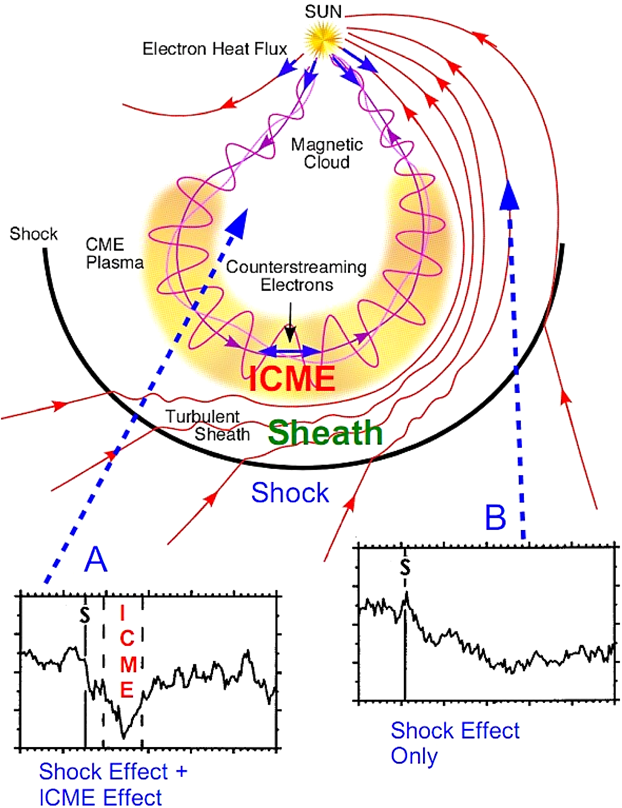
\includegraphics[width=0.6\textwidth]{images/richardson_cane_2011_icme.png}
	\caption{Illustration of an ICME that drives a shock and causes a classical two-step Forbush decrease at location A, where both the shock/sheath and the magnetic cloud pass. At location B, only a single-step Forbush decrease is observed because only the shock is seen here. Source: \citet[Figure 1]{Richardson-Cane-2011}, reprinted by permission from Springer Nature.}
	\label{fig:richardsoncane-cme}
\end{figure}
Typical amplitudes of \acp{FD} can range from a few percent up to more than \SI{10}{\percent} depending on the event, but this varies significantly depending on which particle energies are observed, as lower energy particles are modulated more easily and thus show larger \acp{FD} \citep{Lockwood1971,Lockwood1991}.

% TODO: FD modeling: PDB, ForbMod, ...

\section{Motivation}

To better understand the propagation of \acp{ICME} in the heliosphere, their radial evolution and impacts on Earth, it is essential to make measurements not only in situ at Earth, but from as many locations as possible, to be able to validate and calibrate modeling approaches and thus improve our forecasting capabilities. This includes both in situ measurements at different locations on the \ac{ICME}'s trajectory, e.g. as an upstream monitor to give early warning of an approaching \ac{ICME}, as well as remote sensing observations from the side to better understand the global \ac{CME} characteristics. Measurements at other locations also become increasingly relevant for the large amount of operating and planned space missions (including e.g. human spaceflight to Mars in the next decades), which are also in need of space weather forecasting for safe operations.

While spacecraft with appropriate plasma and magnetic field measurements are available at some locations, it is also sensible to introduce \acp{FD} into the framework of space weather observations, as some missions only carry particle detectors or provide other data only in limited form. For example, the \ac{RAD} instrument on the \ac{MSL} mission, which will be introduced in \autoref{sec:mslrad}, has been and still is the only instrument that provides continuous coverage of space weather at Mars through its \ac{FD} observations --- other missions such as Mars Express (2003) and MAVEN (2014) carry some plasma or magnetic field instruments, but only have limited coverage as their orbits dip into the bow shock of Mars so that the upstream solar wind cannot be observed all the time. This thesis will present the first systematical studies of Forbush decreases at Mars using the \ac{RAD} cosmic ray data.
% TODO: Mehr als nur Ankunftszeit, Überleitung zu HI and SolO

In \autoref{chp:instruments}, an overview of the most important instruments employed in these studies and their data products will be given. The following chapters present several peer-reviewed publications that study \ac{ICME} arrival times at \SI{1}{\AU} and Mars using \acp{FD} and remote sensing observations (\autoref{chp:arrival_times}), additional properties of \acp{FD} at Earth and Mars and their implications for \ac{CME} radial evolution (\autoref{chp:fd_properties}) as well as case studies of a major \ac{SEP} event at Mars that was associated with multiple \acp{ICME} (\autoref{chp:september_event}) and of the first \ac{ICME} and the corresponding \ac{FD} observed at the Solar Orbiter spacecraft (\autoref{chp:solo}). Three appendices follow, which describe certain technical aspects of these studies in more detail, such as the derivation of response functions for the \ac{HET} onboard Solar Orbiter (\autoref{chp:HETSimulation}) and the development of a new software tool implementing of the \ac{GCS} model for the reconstruction of \acp{CME} in remote sensing observations (\autoref{chp:GCS_Python}). Finally \autoref{chp:Publicationlist} presents a list of all publications that I have contributed to, including those that are not included within this PhD thesis as they do not directly fit into the logical flow.
